%----------------------------------------------------------------------------------------
%	PAQUETES
%----------------------------------------------------------------------------------------

\documentclass[12pt,spanish]{article} % Default font size is 12pt, it can be changed here

\usepackage{geometry} % Required to change the page size to A4
\geometry{a4paper} % Set the page size to be A4 as opposed to the default US Letter

\usepackage{graphicx} % Required for including pictures

\usepackage{float} % Allows putting an [H] in \begin{figure} to specify the exact location of the figure
\usepackage{wrapfig} % Allows in-line images such as the example fish picture

\usepackage{lipsum} % Used for inserting dummy 'Lorem ipsum' text into the template

\linespread{1.} % Line spacing

\setlength{\parskip}{0.3cm} % Paragraph vertical spacing

%\setlength\parindent{0pt} % Uncomment to remove all indentation from paragraphs

\graphicspath{{Pictures/}} % Specifies the directory where pictures are stored

% Specify Spanish packages
\usepackage[spanish]{babel}
\selectlanguage{spanish}
\usepackage[utf8]{inputenc}

% Table
\usepackage{tabularx}
\usepackage{array}

\usepackage{caption}

\usepackage{algorithm,refcount}          %  float wrapper for algorithms.
\usepackage{algpseudocode}      % layout for algorithmicx
\usepackage{amsmath}            % AMS mathematical facilities for LATEX
\floatname{algorithm}{Algoritmo}

% Para floor y ceil
\usepackage{mathtools}
\DeclarePairedDelimiter\ceil{\lceil}{\rceil}
\DeclarePairedDelimiter\floor{\lfloor}{\rfloor}

% Para poder usar equation* y tener ecuaciones sin numero
\usepackage{amsmath}

\usepackage[final]{pdfpages}

% Fonts con colores
\usepackage{xcolor}

\definecolor{violeta}{HTML}{400080}
\definecolor{azul}{HTML}{0033CC}
\definecolor{rojo}{HTML}{FF0000}

% Para headers y footers
\usepackage{fancyhdr}
 
\fancyhf{}
\lhead{Puntos Relevantes y Panoramas}
\rhead{Federico Rafael García García}
\cfoot{\thepage}

% Autor y titulo
\author{Federico Rafael García García}

\begin{document}

\abovedisplayshortskip=0pt
\belowdisplayshortskip=0.0cm
\abovedisplayskip=0.0cm
\belowdisplayskip=0pt


%----------------------------------------------------------------------------------------
%	TITLE PAGE
%----------------------------------------------------------------------------------------

\begin{titlepage}

\newcommand{\HRule}{\rule{\linewidth}{0.5mm}} % Defines a new command for the horizontal lines, change thickness here

\center % Center everything on the page

\LARGE Universidad de Granada\\[1cm] % Name of your university/college


\includegraphics[scale=.2]{logo}

\HRule \\[0.5cm]
{ \LARGE \bfseries Práctica 2: Detección de Puntos Relevantes y Construcción de Panoramas}\\[0.1cm] % Title of your document
\HRule \\[0.5cm]

\vspace{1.0cm}

\Large \textbf{Visión por Computador}

\vspace{0.75cm}

\large Federico Rafael García García

\large Curso 2018/2019



{\today} % Date, change the \today to a set date if you want to be precise

%\includegraphics{Logo}\\[1cm] % Include a department/university logo - this will require the graphicx package

\vfill % Fill the rest of the page with whitespace

\end{titlepage}

%----------------------------------------------------------------------------------------
%	INDICE
%----------------------------------------------------------------------------------------

\tableofcontents % Include a table of contents

\newpage % Begins the essay on a new page instead of on the same page as the table of contents 


%----------------------------------------------------------------------------------------
%	EJERCICIO 1
%----------------------------------------------------------------------------------------

\pagestyle{fancy}

\section{Ejercicio 1}


\textbf{
Detección de puntos SIFT y SURF. Aplicar la detección de puntos SIFT y SURF sobre las imágenes, representar dichos puntos sobre
las imágenes haciendo uso de la función drawKeyPoints. Presentar los resultados con las imágenes Yosemite.rar.
}

%----------------------------------------------------------------------------------------
%	EJERCICIO 1.A
%----------------------------------------------------------------------------------------

\subsection{Apartado A}

\textbf{
Variar los valores de umbral de la función de detección de puntos hasta obtener un conjunto numeroso ($\geq$ 1000) de puntos SIFT y SURF que sea representativo de la imagen. Justificar la elección de los parámetros en relación a la representatividad de los puntos obtenidos.
}

Los puntos SIFT consisten en puntos localizados en regiones ``características'' de una imagen; zonas donde hay cambios de intensidades considerables entre píxeles vecinos. Una región ``plana'' como puede ser una pared completamente blanca no se considera de interés, al no tener características visuales que la hagan destacar de otras imágenes. Estos puntos se obtienen creando una pirámide gaussiana de escalas (por cada octava se aplican sucesivos alisamientos gaussianos de diferente escala). En una misma octava se obtienen DoGs (Diferencias Gaussianas) como aproximaciones de Laplacianas (por velocidad) y por cada píxel se compara con sus vecinos 3x3x3 (aparte de los vecinos de la misma escala, los vecinos de la escala superior e inferior) si es un mínimo o un máximo. Cada mínimo o máximo encontrado será un punto de interés.

Estos puntos de interés o \textit{keypoints} pueden ser obtenidos a través de la función \texttt{detect} de un objeto tipo SIFT de OpenCV. Para crear uno llamamos a \texttt{cv2.xfeatures2D.SIFT\_create}. Le pasamos como argumento el número de puntos que deseamos obtener, además de otros parámetros. Hemos dejado por defecto los demás parámetros, que son los siguientes:

\begin{itemize}
\item \texttt{nOctaveLayers}: Por defecto 3 capas por octava.
\item \texttt{sigma}: Cuyo valor inicial es 1,6.
\item \texttt{contrastThreshold}: Como se explicó antes, un punto de interés puede ser obtenido cómo el mínimo o máximo de una región 3x3x3. Algunos mínimos pueden estar poco contrastados con sus vecinos, lo que significaría que no es un punto de interés y deberá ser por tanto descartado. Por defecto 0,4.
\item \texttt{edgeThreshold}: Similar al parámetro anterior, pero filtra puntos cuya región se asemeja a bordes; los bordes no se consideran regiones de interés. Por defecto 10.
\end{itemize}

La razón de haber utilizado estos parámetros por defecto ha sido que los resultados han sido muy buenos sin haberlos cambiado: no han aparecido puntos en las zonas de poco interés, como la sombra que proyecta la montaña o el cielo. El número de octavas no se puede cambiar: las calcula automáticamente SIFT en base al tamaño de la imagen.

SURF consiste en una aproximación de SIFT para mejorar la velocidad, siendo los cambios más destacados el uso de \textit{box filter} en lugar de alisamiento Gaussiano y el uso de una matriz \textit{Hessian}. Esta matriz está formada por los valores de las Laplacianas aproximadas. La matriz \textit{Hessian} dado el punto $p$, escala $\sigma$ y Laplaciana $L_ij$ en direcciones $i$ y $j$ viene dado como sigue:

\[
H
=
\begin{bmatrix}
    L_{xx}(p, \sigma) & L_{xy}(p, \sigma) \\
    L_{yx}(p, \sigma) & L_{yy}(p, \sigma) \\
\end{bmatrix}
\]

El determinante de esta matriz se utiliza para buscar cambios de intensidad alrededor del punto.

Los puntos SURF pueden ser obtenidos a través de la función \texttt{detect} de un objeto tipo SURF. Creamos uno con \texttt{cv2.xfeatures2D.SURF\_create}. Le pasamos como argumento el \textit{threshold} del determinante de la matriz Hessiana: cuanto más alto sea se detectarán menos puntos, pero más característicos. Los parámetros más destacados que recibe son los siguientes:

\begin{itemize}
\item \texttt{nOctaveLayers}: Se ha dejado por defecto a 3.
\item \texttt{nOctave}: El número de octavas utilizado ha sido 3. Según las pruebas realizadas, la 3a octava contiene menos del 3\% del total de puntos obtenidos. No se producirán mejoras en el número de puntos a obtener si se incrementa este parámetro.
\item \texttt{hessianThreshold}: Valor del determinante de la matriz Hessiana para descartar o no puntos. Se explica más adelante los resultados obtenidos según el valor utilizado.

\end{itemize}

Se experimentó con el parámetro de SURF \texttt{hessianThreshold} para la primera imagen. Con valor igual a 100 se han obtenido desmasiados puntos, y algunos no característicos (se pueden ver algunos en el cielo y en la sombra). Con 1000 se obtienen menos puntos de los que pide el enunciado (1000 puntos). Con valor igual a 500 se obtienen más de 1000 puntos y únicamente en la montaña (excepto un único punto en la sombra de Yosemite2); este ha sido el valor utilizado para Yosemite1 y Yosemite2.

Para el caso de SIFT debemos indicar el número de puntos deseados; utilizamos 1000 puntos para ambas imágenes.

En las siguientes imágenes se pueden ver los resultados obtenidos en las imágenes Yosemite1 y Yosemite2, tanto para SIFT como para SURF:

\begin{figure}[H]
  \begin{center}
  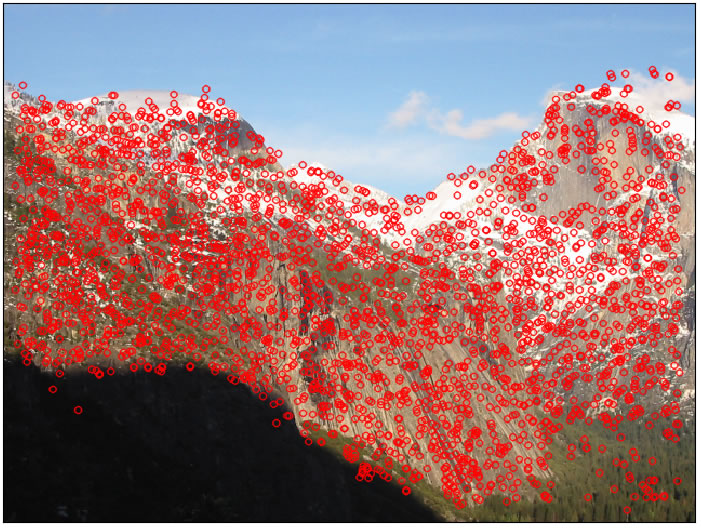
\includegraphics[scale=.6]{ej1_surf1_ht100}
  \caption{Puntos SURF en Yosemite 1 con HT = 100. Se detectaron 2751 puntos}
  \label{fig:ej1_surf1_ht100}
  \end{center}
\end{figure}

\begin{figure}[H]
  \begin{center}
  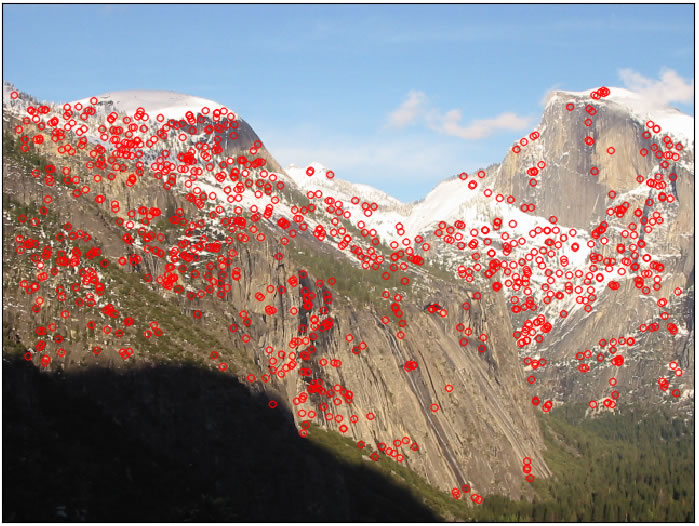
\includegraphics[scale=.6]{ej1_surf1_ht1000}
  \caption{Puntos SURF en Yosemite 1 con HT = 1000. Se detectaron 922 puntos}
  \label{fig:ej1_surf1_ht1000}
  \end{center}
\end{figure}

\begin{figure}[H]
  \begin{center}
  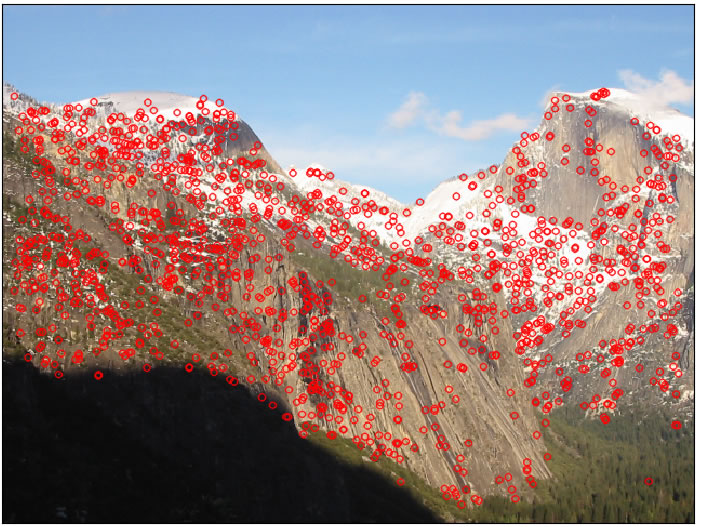
\includegraphics[scale=.6]{ej1_surf1_ht500}
  \caption{Puntos SURF en Yosemite 1 con HT = 500. Se detectaron 1486 puntos}
  \label{fig:ej1_surf1_ht500}
  \end{center}
\end{figure}

\begin{figure}[H]
  \begin{center}
  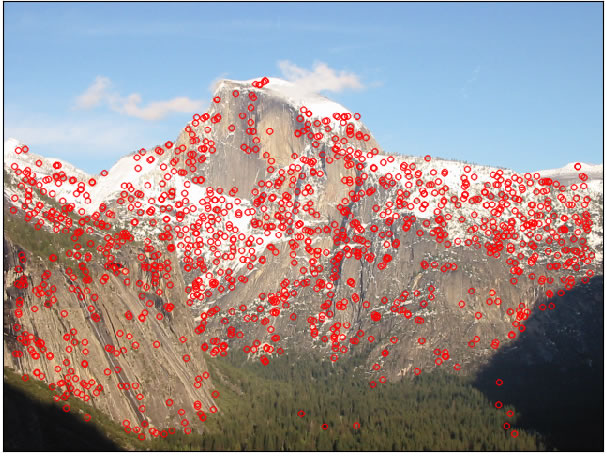
\includegraphics[scale=.6]{ej1_surf2_ht500}
  \caption{Puntos SURF en Yosemite 2 con HT = 500. Se detectaron 1226 puntos}
  \label{fig:ej1_surf2_ht500}
  \end{center}
\end{figure}

\begin{figure}[H]
  \begin{center}
  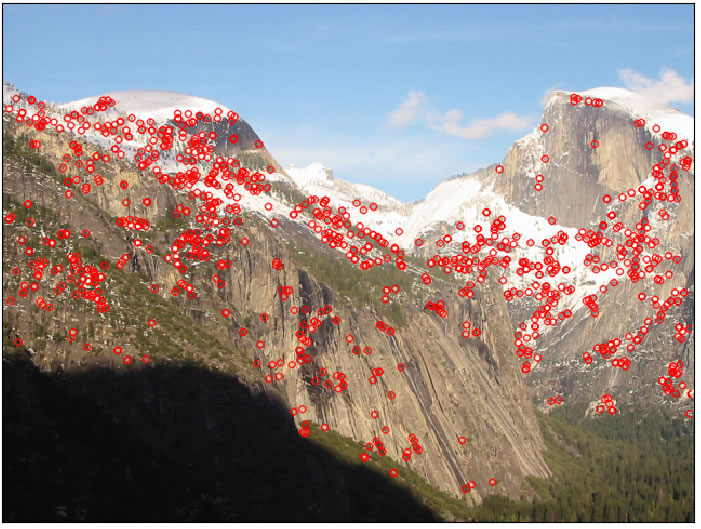
\includegraphics[scale=.6]{ej1_sift1}
  \caption{Puntos SIFT en Yosemite 1. Se detectaron 1000 puntos}
  \label{fig:ej1_sift1}
  \end{center}
\end{figure}

\newpage

\begin{figure}[H]
  \begin{center}
  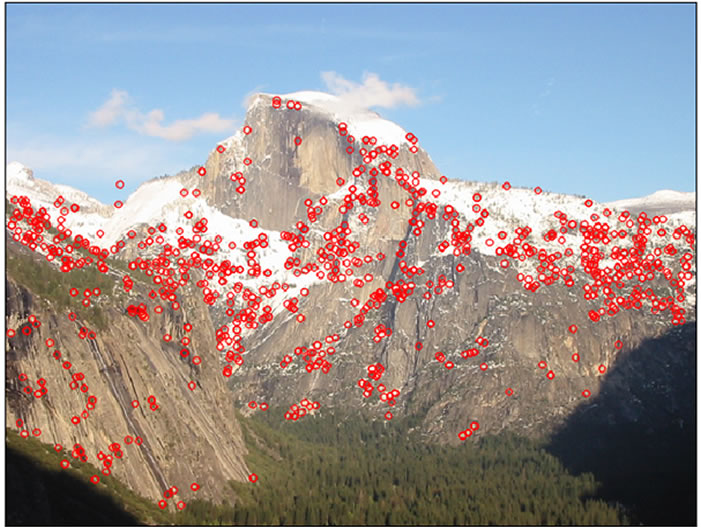
\includegraphics[scale=0.6]{ej1_surf1_ht500-2}
  \caption{Puntos SIFT en Yosemite 2. Se detectaron 1000 puntos}
  \label{fig:ej1_sift2}
  \end{center}
\end{figure}

%----------------------------------------------------------------------------------------
%	EJERCICIO 1.B
%----------------------------------------------------------------------------------------

\subsection{Apartado B}

\textbf{
Identificar cuántos puntos se han detectado dentro de cada octava. En el caso de SIFT, identificar también los puntos detectados en cada capa. Mostrar el resultado dibujando sobre la imagen original un círculo centrado en cada punto y de radio proporcional al valor de sigma usado para su detección (ver circle()) y pintar cada octava en un color.
}

Se han escrito dos funciones para detectar los puntos de cada octava, una para puntos SIFT y otra para puntos SURF, ya que los puntos SIFT contienen más campos que los SURF y han de ser tratados de formas diferentes. En concreto, para los puntos SIFT cada octava está divida en capas, cada cual contendrá puntos.

Las funciones son \texttt{GetKeypointsPorOctavaSIFT} y \texttt{GetKeypointsPorOctavaSURF}; reciben como único parámetro una lista de \textit{keypoints} y devuelven un array de arrays para el caso de SURF (un array con puntos por octava) y un array de arrays de arrays para el caso de SIFT (un array con capas con puntos por cada octava). Para saber el tamaño del array se busca primero la octava más grande.

Para almacenar los puntos, en el caso de SURF basta con acceder al campo \textit{octave} de cada \textit{keypoint} y almacenarlo en el array indicado usando la octava como índice. En el caso de SIFT, se ha de ``desempaquetar'' cada \textit{keypoint}. Resulta que el campo de octava consiste en un entero que contiene además la capa y la escala; este entero ha de ser manipulado mediante desplazamientos de bits para obtener los distintos campos. Para ello se ha utilizado la función \texttt{unpackSIFTOctave}. El código de esta función ha sido obtenido en la página de GitHub de OpenCV [1].

Cabe destacar que mientras la primera octava de SURF es 0 (la imagen original), en SIFT es -1 (la primera octava es una imagen con mayor resolución a la original). Se ha decidido numerar la primera octava como 1 por simplicidad, tanto para SURF como para SIFT, a pesar de que representen realidades diferentes.

En la siguiente tabla se recogen los puntos obtenidos por octava para SURF:

\begin{center}
 \begin{tabular}{|| c | c | c ||} 
 \hline
 \rule{0cm}{0.5cm}
 \textbf{Octava} & \textbf{Puntos Yosemite1} & \textbf{Puntos Yosemite2}  \\
 \hline\hline
 1 & 1161 & 952 \\ 
 \hline
 2 & 255 & 223 \\ 
 \hline
 3 & 70 & 51 \\ 
 \hline\hline
 \textbf{Total} & 1486 & 1226 \\ 
 \hline
\end{tabular}
\end{center}

\newpage

En la siguiente tabla se recogen los puntos obtenidos por octava y capa para SIFT:

\begin{center}
 \begin{tabular}{|| c | c | c | c ||} 
 \hline
 \rule{0cm}{0.5cm}
 \textbf{Octava} & \textbf{Capa} & \textbf{Puntos Yosemite1} & \textbf{Puntos Yosemite2}  \\
 \hline\hline
  1 & 1 & 397 & 435 \\
 \hline
  1 & 2 & 235 & 209 \\
 \hline
  1 & 3 & 141 & 132 \\
  \hline\hline
  2 & 1 & 84 & 91 \\
 \hline
  2 & 2 & 56 & 67 \\
 \hline
  2 & 3 & 34 & 28 \\
  \hline\hline
  3 & 1 & 20 & 14 \\
 \hline
  3 & 2 & 12 & 7 \\
 \hline
  3 & 3 & 5 & 11 \\
  \hline\hline
  4 & 1 & 4 & 3 \\
 \hline
  4 & 2 & 1 & 0 \\
 \hline
  4 & 3 & 4 & 1 \\
  \hline\hline
  5 & 1 & 3 & 0 \\
 \hline
  5 & 2 & 0 & 0 \\
 \hline
  5 & 3 & 0 & 0 \\
  \hline\hline
  6 & 1 & 1 & 1 \\
 \hline
  6 & 2 & 0 & 0 \\
 \hline
  6 & 3 & 0 & 1 \\
  \hline\hline
 \textbf{Total} & & 1000 & 1000 \\ 
 \hline
\end{tabular}
\end{center}

Tanto en SURF como en SIFT, cuanto mayor es el número de octava menor es el número de puntos obtenidos. Esto se debe a que se trata de imágenes pequeñas al haber sido reducidas en mitades múltiples veces; hay menos información de la que obtener puntos (considérese el caso más extremo, el de la octava más pequeña posible, una imagen de 1x1 píxeles). A partir de la cuarta octava apenas se obtienen puntos.

Podemos pintar los puntos por encima de la imagen de la cual han sido extraídos. Las octavas han sido codificadas por color. Según el paper de Lowe, el sigma utilizado en cada octava es el doble de la anterior. Se ha utilizado un sigma inicial de 1.6, el que utiliza OpenCV por defecto. Definimos el radio de cada círculo como 3 veces sigma. El algoritmo de SURF es diferente al de SIFT: en lugar de utilizar alisamiento gaussiano, utiliza un \textit{box filter} como aproximación (de esta manera consigue resultados más rápidos). Según la documentación leída sobre SURF, se utiliza un sigma inicial de 1.2: este es el valor que se ha utilizado.

En las siguientes imágenes se pueden ver los resultados obtenidos en las imágenes Yosemite1 y Yosemite2, tanto para SIFT como para SURF:

\begin{figure}[H]
  \begin{center}
  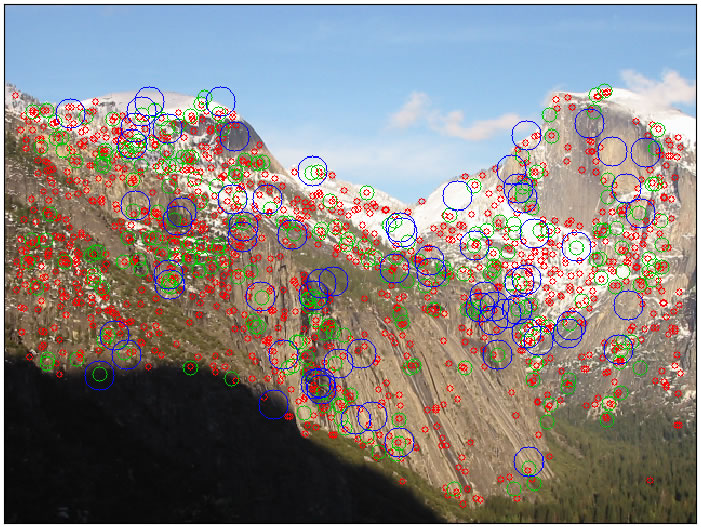
\includegraphics[scale=.6]{ej1_surf1_octavas}
  \caption{Puntos SURF en Yosemite 1. Octavas: 1=Rojo, 2=Verde, 3=Azul}
  \label{fig:ej1_surf1_octavas}
  \end{center}
\end{figure}

\begin{figure}[H]
  \begin{center}
  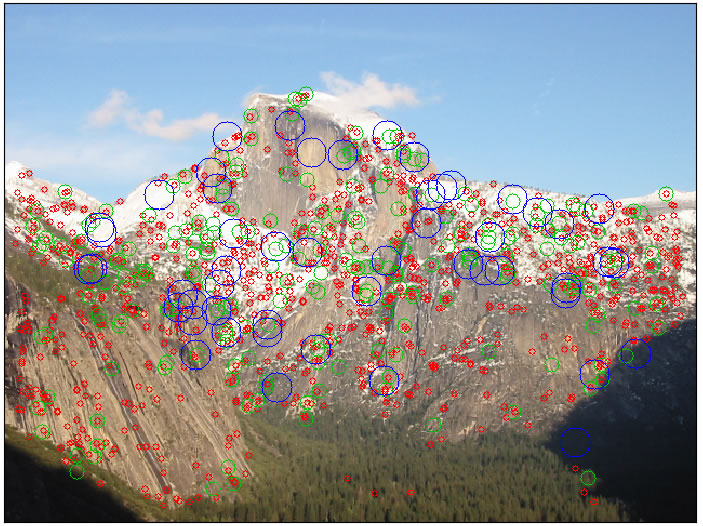
\includegraphics[scale=.6]{ej1_surf2_octavas}
  \caption{Puntos SURF en Yosemite 2. Octavas: 1=Rojo, 2=Verde, 3=Azul}
  \label{fig:ej1_surf2_octavas}
  \end{center}
\end{figure}

\begin{figure}[H]
  \begin{center}
  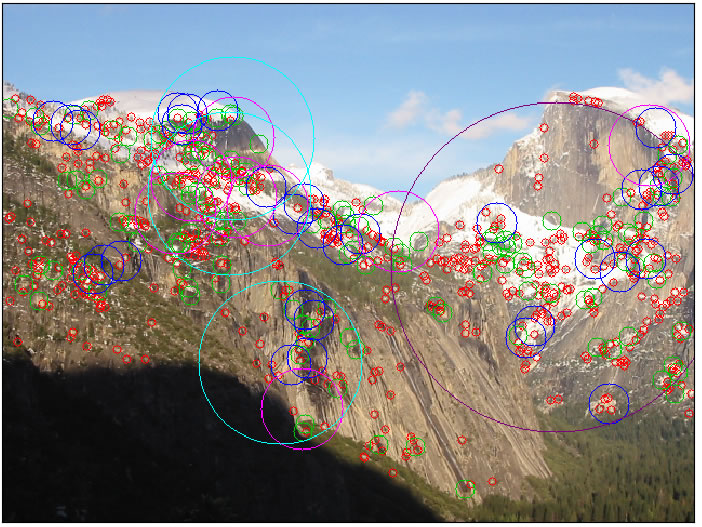
\includegraphics[scale=.6]{ej1_sift1_octavas}
  \caption{Puntos SIFT en Yosemite 1. Octavas: 1=Rojo, 2=Verde, 3=Azul, 4=Cyan, 5=Magenta, 6=Violeta}
  \label{fig:ej1_sift1_octavas}
  \end{center}
\end{figure}

\begin{figure}[H]
  \begin{center}
  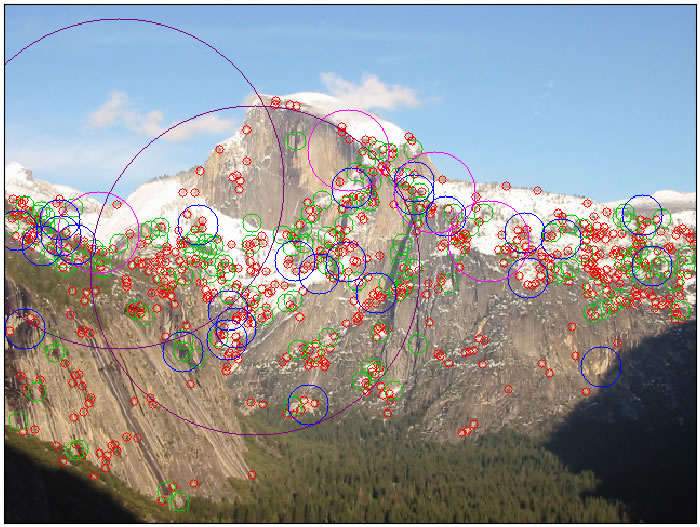
\includegraphics[scale=.6]{ej1_sift2_octavas}
  \caption{Puntos SIFT en Yosemite 2. Octavas: 1=Rojo, 2=Verde, 3=Azul, 4=Cyan, 5=Magenta, 6=Violeta}
  \label{fig:ej1_sift2_octavas}
  \end{center}
\end{figure}

%----------------------------------------------------------------------------------------
%	EJERCICIO 1.C
%----------------------------------------------------------------------------------------

\subsection{Apartado C}

\textbf{
Mostrar cómo con el vector de keyPoint extraídos se pueden calcular los descriptores SIFT y SURF asociados a cada punto usando OpenCV.
}

Con los puntos obtenidos en los apartados anteriores, podemos obtener sus descriptores llamando a la función \texttt{compute} de cada objeto SURF o SIFT pasando como argumentos la imagen y la lista de \textit{keypoints} extraídos de dicha imagen.

Un descriptor consiste en una ventana de 16x16 (vecinos alrededor del punto). Esta ventana se divide en bloques de 4x4. Mediante cálculo de gradientes, para cada píxel se obtiene una dirección. De cada bloque 4x4 se agrupan las direcciones en 8 posibles. Este descriptor permite identificar a un punto de los demás.

\newpage

%----------------------------------------------------------------------------------------
%	EJERCICIO 2
%----------------------------------------------------------------------------------------

\section{Ejercicio 2}

\textbf{
Usar el detector-descriptor SIFT de OpenCV sobre las imágenes de Yosemite.rar (cv2.xfeatures2d.SIFT\_create()). Extraer sus listas de keyPoints y descriptores asociados. Establecer las correspondencias existentes entre ellos usando el objeto BFMatcher de OpenCV y los criterios de correspondencias ``BruteForce+crossCheck'' y ``Lowe-Average-2NN''. (NOTA: Si se usan los resultados propios del puntos anterior en lugar del cálculo de SIFT de OpenCV se añaden 0.5 puntos)
}

\subsection{Apartado A}

\textbf{
Mostrar ambas imágenes en un mismo canvas y pintar líneas de diferentes colores entre las coordenadas de los puntos en correspondencias. Mostrar en cada caso 100 elegidas aleatoriamente
}

En las siguientes figuras se ven los resultados:

\begin{figure}[H]
  \begin{center}
  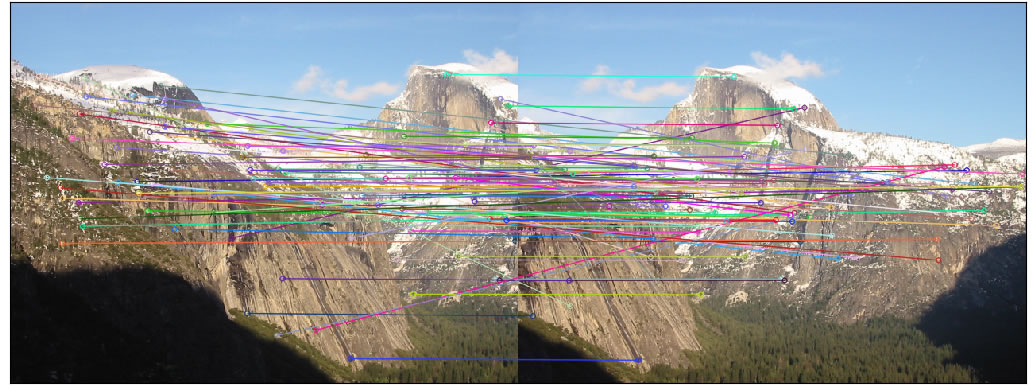
\includegraphics[scale=.6]{ej2_bf}
  \caption{Correspondencias en Yosemite con Bruteforce+crossCheck}
  \label{fig:ej2_bf}
  \end{center}
\end{figure}

\begin{figure}[H]
  \begin{center}
  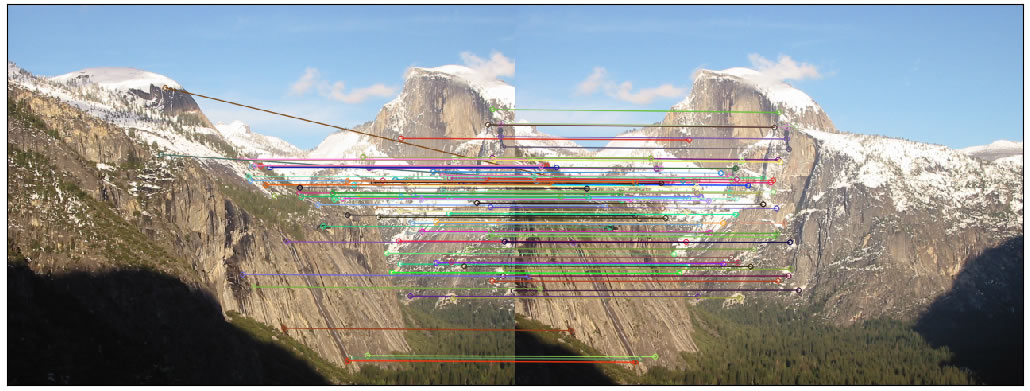
\includegraphics[scale=.6]{ej2_2nn}
  \caption{Correspondencias en Yosemite con Lowe 2NN}
  \label{fig:ej2_2nn}
  \end{center}
\end{figure}

\subsection{Apartado B}

\textbf{
Valorar la calidad de los resultados obtenidos en términos de las correspondencias válidas observadas por inspección ocular y las tendencias de las líneas dibujadas.
}

Los puntos y descriptores los hemos obtenido en el ejercicio anterior. Para obtener las correspondencias entre los puntos de Yosemite1 y Yosemite2 utilizamos dos técnicas: ``BruteForce+crossCheck'' y ``Lowe-Average-2NN''.

\textit{BruteForce}, del inglés ``Fuerza bruta'', consiste en comparar el descriptor de cada punto de la primera imagen con el de la segunda para obtener la mejor correspondencia. La opción \textit{crossCheck}, del inglés ``Chequeo cruzado'', consiste en comparar cada punto de la segunda imagen con el de la primera; puede ocurrir que un punto $P$ de la primera imagen se corresponda mejor con punto $P'$ de la segunda imagen, pero que $P'$ no se corresponda con $P$. El \textit{crossCheck} realiza esta comprobación, con el fin de generar mejores correspondencias.

\textit{Lowe-Average-2NN} consiste en seleccionar por cada punto de la primera imagen los dos puntos que tengan mejor correspondenca en la segunda imagen. Luego se aplica el \texttt{Ratio test} de Lowe: cuanto más se aproxime el ratio a 1, más similares son los puntos.

Se utilizó un ratio igual a 0,75.

Una vez obtenidos los puntos para cada \textit{matcher}, se seleccionaron 100 al azar y se pintaron las correspondencias de los puntos de la primera imagen con la segunda mediante líneas.

Se puede ver una gran cantidad de \textit{outliers} con el BruteForce matcher, es decir, correspondencias erróneas entre puntos (muchas líneas de correspondencias se cruzan). Esto se debe a que dos descriptores parecidos no necesariamente tienen que corresponderse con las mismas regiones de dos puntos. Esto resultará en correspondencias equivocadas y, por tanto, una mala calidad en los resultados.

El test de ratio de Lower soluciona ese problema; solo se puede ver un único outlier, el resto de las línas de correspondencia son paralelas. Esto se debe a que si las dos mejores correspondencias están muy cerca entre ellas la probabilidad de que sea una correspondencia de regiones correcta es elevada.


\subsection{Apartado C}

\textbf{
Comparar ambas técnicas de correspondencias en términos de la calidad de sus correspondencias (suponer 100 aleatorias e inspección visual).
}

Claramente la calidad de Lowe supera con creces al de BruteForce. El test de ratio ayuda a descartar correspondencias equivocadas que BruteForce da por buenas. Además, al no utilizar crossCheck se obtienen resultados más rápidos.

En conclusión: Lowe no solo ofrece más calidad en los resultados, sino que también en menos tiempo.

%----------------------------------------------------------------------------------------
%	EJERCICIO 3
%----------------------------------------------------------------------------------------

\section{Ejercicio 3}

\textbf{Escribir una función que genere un mosaico de calidad a partir de N = 3 imágenes relacionadas por homografías, sus listas de keyPoints calculados de acuerdo al punto anterior y las correspondencias encontradas entre dichas listas. Estimar las homografías entre ellas usando la función cv2.findHomography(p1, p2, CV\_RANSAC, 1).}

Dado que se utiliza la bandera \texttt{BORDER\_TRANSPARENT}, surgieron problemas de visualización. Al ser las imágenes RGB, se producía ruido en el mosaico resultante. Este problema se solucionó utilizando imágenes en RGBA, que utiliza el canal \textit{alfa} para las transparencias.

\subsection{Apartado A}

\textbf{
Definir una imagen en la que pintaremos el mosaico.
}

La función \texttt{GenerarMosaico} recibe un conjunto de imágenes para generar un mosaico. Estas imágenes se pintan centradas en un \textit{canvas}, que no es más que una imagen muy grande cuyos valores iniciales de sus píxeles son todos 0 (incluida la transparencia). El tamaño de este canvas es la suma de las longitudes de cada imagen y la suma de las alturas: de esta manera se asegura que hay espacio de sobra para colocar todas las imágenes.

Una vez se pintan todas las imágenes en el canvas, se recortan los bordes llamando a la función \texttt{Recortar}. Esta función busca columnas de izquierda a derecha y de derecha a izquierda y filas de arriba a abajo y abajo a arriba cuyos valores de alfa sean distintos de 0; esto significaría que se ha llegado al comienzo de la imagen. Se marcan estas posiciones y se devuelva la imagen contenida entre esos límites.

\subsection{Apartado B}

\textbf{
Definir la homografía que lleva cada una de las imágenes a la imagen del mosaico.
}

Una homografía es una matriz 3x3 que define una transformación geométrica: permite transformar una imagen para rotarla, cambiar su posición, proyección, escala, etc. Pero a diferencia de una mera matriz de transformación, una homografía define la transformación que se debe aplicar para ``llevar'' los puntos de una imagen a otra.

Para calcularla, definimos la función \texttt{GetHomografia}. Recibe dos imágenes y calcula sus puntos y descriptores SIFT: se obtienen 1000 puntos. De estos obtenemos correspondencias buenas aplicando Lowe 2NN. Finalmente, se llama a la función \texttt{cv2.findHomography(p1, p2, CV\_RANSAC, 1)} para obtener la homografía, donde $p1$ y $p2$ son los puntos en correspondencia de cada imagen.

RANSAC es un algoritmo para eliminar outliers. Comprueba cuál es la línea de tendencia de los puntos. Los puntos que estén más alejados de esta línea de tendencia son descartados.

\subsection{Apartado C}

\textbf{
Usar la función cv2.warpPerspective() para trasladar cada imagen al mosaico (Ayuda: Usar el flag BORDER\_TRANSPARENT de warpPerspective).
}

Una vez se ha creado el mosaico vacío en la función \texttt{GenerarMosaico}, procedemos a calcular homografías y pintar las imágenes en el mosaico con \texttt{warpPerspective}, pasándole como fuente una imagen junto con su homografía y el mosaico como imagen de destino donde se pintará. Primero se calculan todas las homografías y se almacenan en un array, y luego se llevan las imágenes al mosaico.

Definimos la homografía identidad H. A esta matriz modificamos las posiciones [0, 2] y [1, 2], responsables de realizar traslaciones, con la mitad de la suma del tamaño del canvas y de la imagen en el medio de la lista de imágenes. Al aplicar esta homografía a dicha imagen, se traslada la imagen al centro del canvas. Guardamos esta matriz en la posición central del array de homografías y en H.

Luego calculamos homografías de cada pareja por la izquierda. Dado que se tratan de matrices de transformación, calculamos la homografía de la imagen de la izquierda del centro con esta y la multiplicamos por H: esto permite que la aplicación de la homografía sea relativa a la posición actual. Guardamos la matriz en la posición correspondiente del array. En un bucle se repite el proceso con todas las imágenes por la izquierda, actualizando H, que es multiplicada por las nuevas homografías.

Se aplica la misma metodología pero con las imágenes por la derecha. Antes de calcular las homografías por la derecha, debemos darle a H el valor inicial, el de la homografía de la imagen central.

En lugar de calcular la homografía de una imagen con la siguiente, se calcula la homografía inversa, la de la imagen siguiente con la actual. Esto se debe a que nos interesa ``traer'' la siguiente imagen al mosaico, y no al revés.

En la figura \ref{fig:panorama1} se ve un mosaico formado por tres imágenes de Yosemite.

\begin{figure}[H]
  \begin{center}
  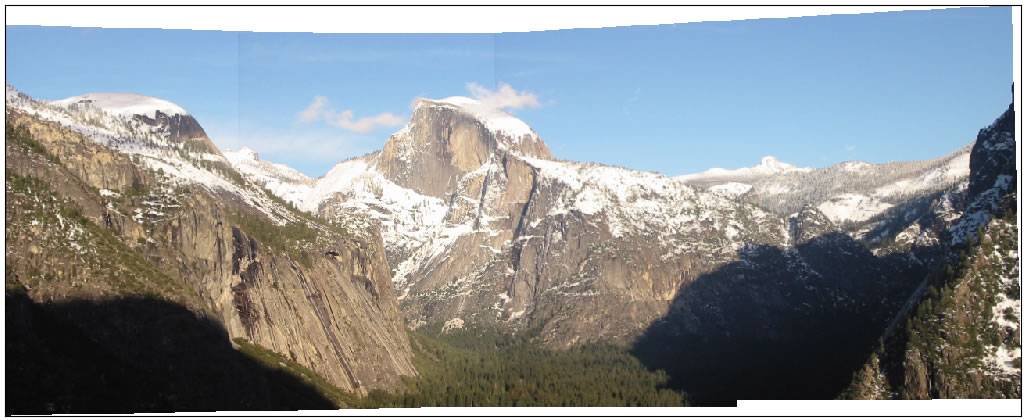
\includegraphics[scale=.55]{panorama1}
  \caption{Panorama formado por imágenes ``Yosemite''. N=3}
  \label{fig:panorama1}
  \end{center}
\end{figure}

El mosaico obtenido es de bastante calidad, aunque existen algunos saltos de intensidad entre las imágenes (notablemente en el cielo). Se pueden ver además las deformaciones en los extremos debido a las proyecciones. Esta es la razón por la cual se utiliza como imagen de partida la central. De lo contrario, la deformación por la izquierda o por la derecha sería demasiado grande como para poder tener un mosaico de calidad.

%----------------------------------------------------------------------------------------
%	EJERCICIO 4
%----------------------------------------------------------------------------------------

\section{Ejercicio 4}

\textbf{Lo mismo que en el punto anterior pero para N $>$ 5 (usar las imágenes para mosaico).}

Se ejecutó la misma función de generación de mosaico que en el apartado anterior, pero con todas las imágenes ``mosaico''.

En la figura \ref{fig:panorama2} se ve el resultado.

\begin{figure}[H]
  \begin{center}
  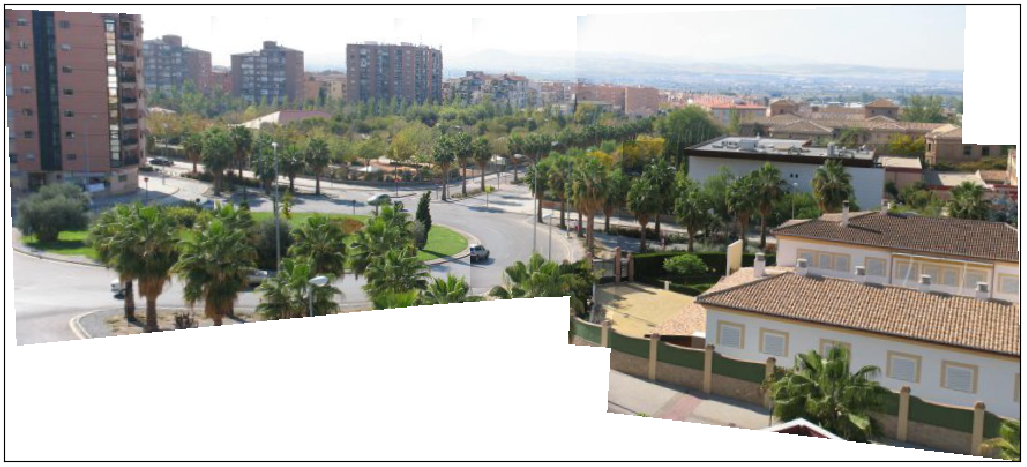
\includegraphics[scale=.55]{panorama2}
  \caption{Panorama formado por imágenes ``mosaico''. N=10}
  \label{fig:panorama2}
  \end{center}
\end{figure}

El mosaico es de bastante calidad, aunque al igual que en el ejercicio anterior se pueden ver saltos de intensidad en los bordes de las imágenes unidas. También se puede ver que un coche ha sido cortado por la mitad, fruto de no haber tomado todas las fotos al mismo tiempo. Aún así las imágenes han quedado correctamente unidas en correspondencia.

%----------------------------------------------------------------------------------------
%	REFERENCIAS
%----------------------------------------------------------------------------------------
\newpage

\section{Referencias}

\noindent
[1] SIFT Octave bug
\\
{\#}4554. \texttt{URL: https://github.com/opencv/opencv/issues/4554}


\section{Bibliografía}

\noindent
David G. Lowe.
\\
\textit{Distinctive Image Features from Scale-Invariant Keypoints}.

\noindent
Herbert Bay, Tinne Tuytelaars and Luc Van Gool.
\\
\textit{SURF: Speeded Up Robust Features}.

\noindent
\textit{Introduction to SIFT.}
\\
\texttt{URL: https://docs.opencv.org/3.4/da/df5/tutorial\_py\_sift\_intro.html}

\noindent
\textit{Introduction to SURF.}
\\
\texttt{URL: https://docs.opencv.org/3.0-beta/doc/py\_tutorials/}
\\
\texttt{py\_feature2d/py\_surf\_intro/py\_surf\_intro.html}

\noindent
\textit{Basic concepts of the homography explained with code.}
\\
\texttt{https://docs.opencv.org/3.4/d9/dab/tutorial\_homography.html}

\noindent
\textit{Feature Matching + Homography to find Objects.}
\\
\texttt{URL: https://docs.opencv.org/3.0-beta/doc/py\_tutorials/}
\\
\texttt{py\_feature2d/py\_feature\_homography/py\_feature\_homography.html}

\noindent
\textit{Speeded up robust features}
\\
\texttt{URL: https://en.wikipedia.org/wiki/Speeded\_up\_robust\_features}

%----------------------------------------------------------------------------------------
%	FIN DEL DOCUMENTO
%----------------------------------------------------------------------------------------

\end{document}